% !TEX root = main.tex
% !TeX spellcheck = en_US

\subsection{Left-Balanced Trees}\label{sec:addleafprf}
In this section, we formally define $q$-ary trees used by \saik to implement ratchet trees.

\begin{definition}[LBT]\label{def:lbt}
	For $\treeArity,n\in\N$ with $q>1$, the \emph{$n$\th left-balanced $\treeArity$-ary tree (LBT)}, denoted $\lbt{\treeArity}{n}$, is defined as follows. $\lbt{\treeArity}{1}$ is the tree consisting of one node.
	For $n>1$, if $m = \max\{\treeArity^p : p \in \N \land \treeArity^p < n\}$ and $k = \lfloor n/m \rfloor$, then $\lbt{\treeArity}{n}$ is the tree whose root has the first $k$ children equal to  $\lbt{\treeArity}{m}$ and, if $n-mk>0$, the $(m+1)$-st child equal to $\lbt{\treeArity}{n-mk}$.
\end{definition}
\begin{definition}[Full LBT]
  For $\treeArity,n\in\N$, $\lbt{\treeArity}{n}$ is full if $n$ is a power of $\treeArity$.
\end{definition}

Operation of \saik requires a procedure $\addleaf(\tree, v)$ which inserts a leaf $v$ into a ratchet tree $\tree$ while preserving certain properties of $\tree$. In particular, $\addleaf$ should preserve node indices $v.\nodeIndex$. They are computed as follows: all nodes are numbered left to right --- i.e., according to an in-order depth-first traversal of the tree ---  starting with $0$. See \cref{fig:lbbtex} for an example.

\begin{figure}[htb]
	\newcommand{\leafindex}[1]{(#1)}
	\newcommand{\nodeindex}[1]{{\color{black}#1}}
	\centering
	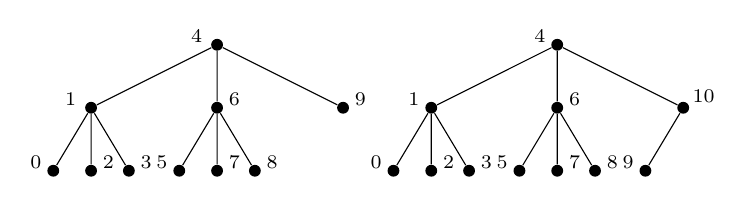
\begin{tikzpicture}[level distance=8mm, xscale = .8]
		\tikzstyle{every node}=[fill=black,circle,minimum size=.15cm,inner sep=0pt]
		\tikzstyle{every label}=[fill=none,font=\scriptsize,draw=none]
		\tikzstyle{level 1}=[sibling distance=20mm]
		\tikzstyle{level 2}=[sibling distance=6mm]
		\tikzstyle{level 3}=[sibling distance=6mm]
    \def\x{.6mm}

		\node[label={[label distance=1mm]170:
			{\nodeindex{4}}
		}] {}
		child {node[label={[label distance=1mm]170:
				{\nodeindex{1}}
			}] {}
			child {node[label={[label distance=\x]170:{\nodeindex{0}}}] {}}
			child {node[label={[label distance=\x]10:{\nodeindex{2}}}] {}}
			child {node[label={[label distance=\x]10:{\nodeindex{3}}}] {}}
		}
		child {node[label={[label distance=\x]10:
				{\nodeindex{6}}
			}] {}
			child {node[label={[label distance=\x]170:{\nodeindex{5}}}] {}}
			child {node[label={[label distance=\x]10:{\nodeindex{7}}}] {}}
			child {node[label={[label distance=\x]10:{\nodeindex{8}}}] {}}
		}
    child {node[label={[label distance=\x]10:
				{\nodeindex{9}}
			}] {}
		};
    \node[label={[label distance=\x]170:
			{\nodeindex{4}}
		}] at (5.4,0) {}
		child {node[label={[label distance=\x]170:
				{\nodeindex{1}}
			}] {}
			child {node[label={[label distance=\x]170:{\nodeindex{0}}}] {}}
			child {node[label={[label distance=\x]10:{\nodeindex{2}}}] {}}
			child {node[label={[label distance=\x]10:{\nodeindex{3}}}] {}}
		}
		child {node[label={[label distance=\x]10:
				{\nodeindex{6}}
			}] {}
			child {node[label={[label distance=\x]170:{\nodeindex{5}}}] {}}
			child {node[label={[label distance=\x]10:{\nodeindex{7}}}] {}}
			child {node[label={[label distance=\x]10:{\nodeindex{8}}}] {}}
		}
    child {node[label={[label distance=\x]10:
				{\nodeindex{10}}
			}] {}
      child {node[label={[label distance=\x]170:{\nodeindex{9}}}] {}}
      child {node[fill=none] {} edge from parent[draw=none]}
      child {node[fill=none] {} edge from parent[draw=none]}
		};
	\end{tikzpicture}
	\caption{The trees $\lbt{3}{7}$ (left) and $\lbt{3}{8}$ (right) with node indices.}
	\label{fig:lbbtex}
\end{figure}

\begin{definition}[$\addleaf$]\label{def:addleaf}
	The algorithm $\addleaf(\tree, v)$ takes as input a $\treeArity$-ary tree $\tree$ with root $r$ and $n$ nodes, and a fresh leaf $v$ and returns a new tree $\tree'$ with $v$ inserted and $v.\nodeIndex=n+1$.
	\begin{enumerate}[label=\alph*),itemsep=0pt]
    \item If $\tree$ is full, then create a new root $r'$ for $\tree'$. Attach $r$ as the first child of $r'$ and $v$ as the second child.
    \item Else if $r.\children$ contains only nodes with full subtrees, let $\tree'=\tree$ except $v$ is attached as the next child of $r$.
    \item Else, let $u$ be the first in $r.\children$ s.t. its subtree $\tree_u$ is not full. Let $\tree'=\tree$ except $\tree_u$ is replaced by $\addleaf(\tree_u,v)$.
	\end{enumerate}
\end{definition}

The following lemma formalizes the correctness of $\addleaf$. We prove it in \cref{sec:addleafprf}.
\begin{restatable}{theorem}{addleafLem}\label{lemm:addleaf}
	$\tree = \lbt{\treeArity}{n} \implies \addleaf(\tree, v) = \lbt{\treeArity}{n+1}$.
\end{restatable}

\begin{proof}
  The proof is by strong induction on $n$. If $n<\treeArity$, then the statement easily follows by inspection (only cases a) and b) of $\addleaf$ apply).
  Fix $n\geq\treeArity$ and assume the statement holds for all $k<n$. Let $r$ be the root of $\tree$ and let $\mpow(n) = \max\{\treeArity^p + 1 : p \in \N \land \treeArity^p < n\}$.

  If $\tree$ is full, then $\mpow(n+1)=n$. Furthermore, the root of $\tree'$ has only two children: $\tree=\lbt{\treeArity}{n} = \lbt{\treeArity}{\mpow(n+1)}$ and $\lbt{\treeArity}{1}$, so $\tree'=\lbt{\treeArity}{n+1}$ per definition.

  Else, $\mpow(n)=\mpow(n+1)$ (this holds since $n\geq\treeArity$). Moreover, it is easy to see that only the last node in $r.\children$ can be non-full. This means that the root $r'$ of $\tree'$ has the following children (in order):
  \begin{itemize}
    \item All children of the root $r$ of $\tree$ which have full subtrees. These subtrees are equal to $\lbt{\treeArity}{\mpow(n)}=\lbt{\treeArity}{\mpow(n+1)}$.
    \item If $r$ has no non-full subtrees, then the last child of $r'$ is $v$ with subtree $\lbt{\treeArity}{1}$.
    \item Else if the last child $u$ of $r$ is non-full and equals to $\lbt{\treeArity}{x}$ for $x<\mpow(n)$, then the last child of $r'$ is $\lbt{\treeArity}{x+1}$ by induction hypothesis.
  \end{itemize}
  Clearly, $\tree'=\lbt{\treeArity}{n+1}$ in all cases.
\end{proof}